\section{State of the art}

A crucial phase in the software development process is the \textit{testing}, which encompasses a suite of methods aimed to verify whether the actual software product aligns with the expected requirements. Software testing serves as an effective means of uncovering bugs within the software. Extensive research has been conducted in recent years to formulate novel testing approaches. While software bugs are typically associated with coding or design errors, in the context of MLMs, bugs are not exclusively due to coding issues. Nonetheless, the goal of the testing phase remains the same: to check if the model meets to the specified requirements. Consequently, MLMs testing focuses around evaluating certain desired properties instead of singular bugs. Currently, the state of the art defines the following properties: \textit{correctness, relevance, robustness, security, privacy, efficiency, fairness and Interpretability} \cite{zhang2019machine}.

However, owing to the intricate nature and increased complexity of these models, conventional software testing techniques are often inapplicable \cite{VVinef}. This limitation becomes particularly significant in safety-critical applications, where quantifying the deviation of actual model qualities from the desired ones becomes crucial. As a result, a wide research has been directed towards pioneering new testing techniques tailored to MLMs. \Fig~\ref{fig:model_dev_wf} provides an overview on how the development process has evolved. Specifically, \Fig~\ref{fig:basic_model_dev} delineates the fundamental workflow for MLMs development, which proved to be effective for simple tasks and non-critical domains. Indeed it does not take into account any testing operation.

Within the MLM development context, there are two primary sources of errors: the data and the model. Errors coming from each source can be attributed to either implementation or design issues. Traditional testing techniques can partially detect implementation errors like code defects. Therefore, MLMs testing encompasses these software techniques and extends their application to address novel challenges. \Fig~\ref{fig:tnv_model_dev} shows the transformation of the basic MLMs development workflow to incorporate testing. This work specifically faces \textit{model} testing.

\begin{figure}[h]
	\centering
	\begin{subfigure}{.5\textwidth}
		\centering
		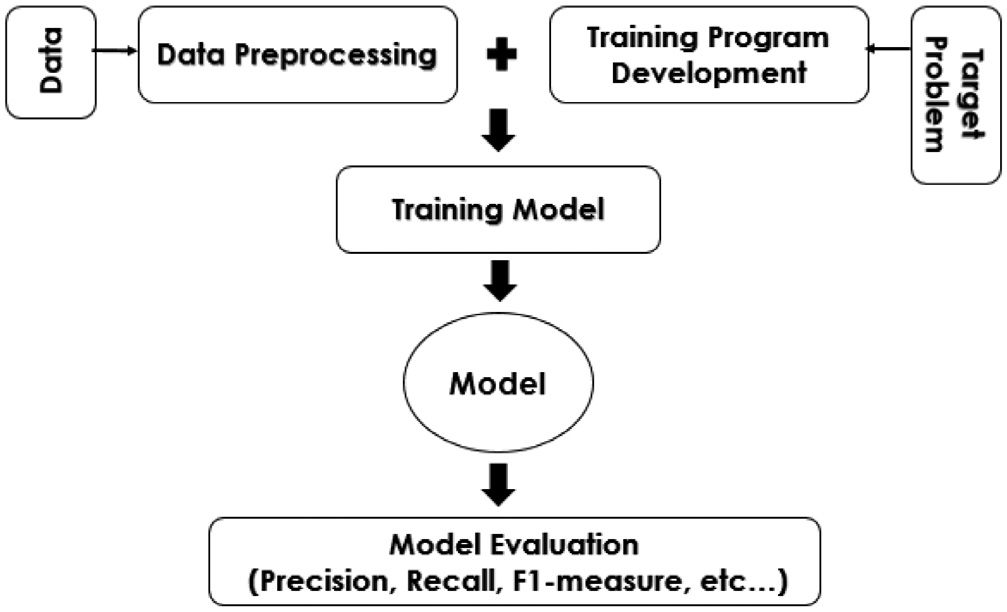
\includegraphics[width=0.8\linewidth]{ImageFiles/StateOfArt/basic_model_dev}
		\caption{Machine learning model development workflow}
		\label{fig:basic_model_dev}
	\end{subfigure}%
	\begin{subfigure}{.5\textwidth}
		\centering
		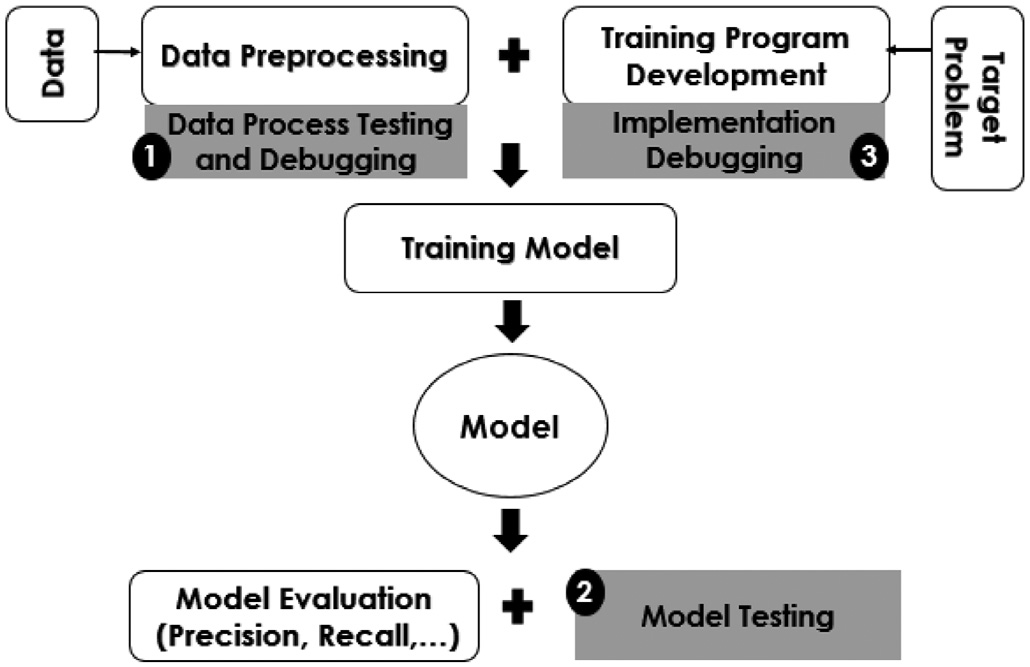
\includegraphics[width=0.8\linewidth]{ImageFiles/StateOfArt/tnv_model_dev}
		\caption{Machine learning model development workflow including the testing phase}
		\label{fig:tnv_model_dev}
	\end{subfigure}
	\caption{Machine learning model development workflow \cite{BRAIEK2020110542}}
	\label{fig:model_dev_wf}
\end{figure}

Model testing can be approached in two primary ways: white-box and black-box methods. White-box testing leverages the model internal structure, including its mathematical formulation. In contrast, black-box testing focuses solely on the input-output behavior, without looking into the internal workings of the model. In general, white-box methods have the potential to enhance testing quality, as they draw from a more comprehensive set of information. However, obtaining access to the internal structure of the model is not always possible. Additionally, black-box methods often demand less effort, making them more straightforward to implement compared to white-box techniques.

As mentioned earlier, MLMs testing centers around evaluating specific desired properties. In this context, the main emphasis of MLMs testing is on the evaluation of the robustness property \cite{Marijan_2020}. Robustness pertains to the model capability to maintain satisfactory performance even in the presence of new operating conditions that were not anticipated during the design phase.

Before giving the definition of robustness it is necessary to introduce the concept of correctness, which measures the probability that a MLM gives the right output. More formally, let $x$ be a sample belonging to the future unknown data distribution $D$. Let $h$ be the MLM under test. $h(x)$ denotes the predicted label for the sample $x$, while $c(x)$ denotes the true label. The model correctness $E(h)$ is defined as the probability that $h(x)$ and $c(x)$ are identical:
\[
	E(h)  = Pr_{x\sim D}[h(x) = c(x)]
\]

Achieving a high model correctness is a fundamental goal in machine learning, as it determines the practical utility and effectiveness of the model. 

Let's now proceed to formally define robustness: Let $S$ be the MLM under test. Let be $\delta (S)$ the MLM $S$ subject to some perturbations. The robustness of a MLM $S$ is defined as:

\[
	r = E(S) - E(\delta (S))
\]

In simpler terms, the robustness metric measures how much the performance deteriorates when the operating conditions deviate from the nominal ones.

In this study, the primary approach employed will be black-box testing, with a specific emphasis on evaluating robustness. More precisely, novel methods will be introduced to assess the robustness of a BNN by exploiting the estimated uncertainty.